\begin{frame}{\makebox[0pt][l]{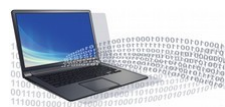
\includegraphics[scale=0.3]{Logotip.png}}\hspace{5.5cm}\textbf{\textcolor{blue}{П}\textcolor{gray}{риставки для единиц измерения\\\hspace{4cm}количества информации/данных: проблема}}}

    \fontsize{11pt}{13pt}\selectfont
    \hspace{2cm}Linux Ubuntu 14 \hspace{2.7cm}Microsoft Windows 7

    \begin{figure}
        \centering
        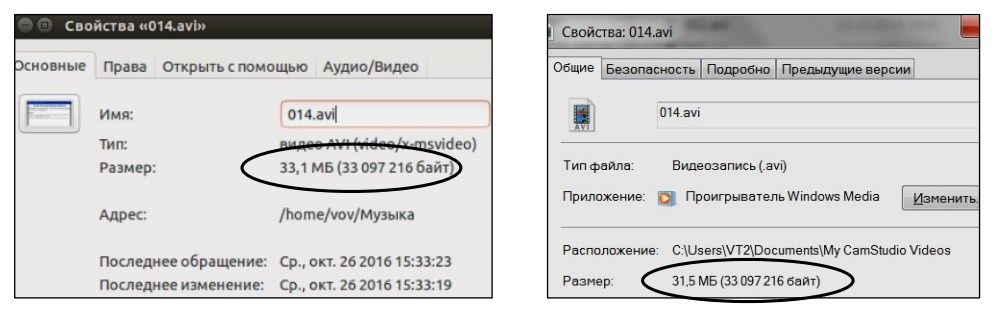
\includegraphics[scale =0.4]{Slide21.png}
    \end{figure}
    
    \medskip
    \fontsize{11pt}{13pt}\selectfont
    \hspace{2.5cm}33 097 216 байт — это \textcolor{Green}{33,1} МБ или \textcolor{Green}{31,5} МБ?
    
\end{frame}
